\begin{figure}[h]
	\centering
	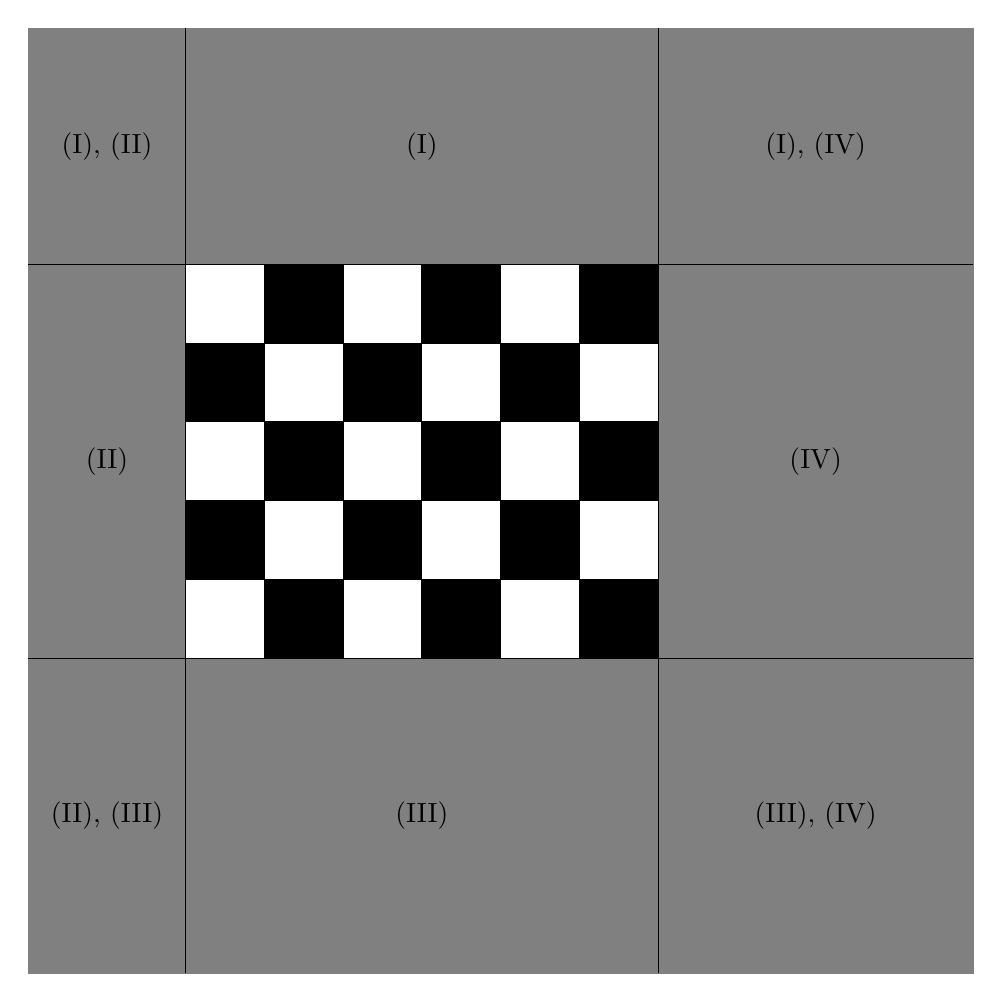
\begin{tikzpicture}
		\foreach \i in {-6, ..., 5}
			\foreach \j in {-6, ..., 5}
				\filldraw[gray] (\i, \j) rectangle + (1, 1);
		\foreach \i in {-4, ..., 1}
			\foreach \j in {-2, ..., 2}
			{
				\pgfmathparse{mod(\i+\j, 2) ? "black" : "white"}
				\edef\colour{\pgfmathresult}
				\filldraw[fill=\colour] (\i, \j) rectangle + (1, 1);
			}
		\draw (-4, -6) -- (-4, 6);
		\draw (2, -6) -- (2, 6);
		\draw (-6, -2) -- (6, -2);
		\draw (-6, 3) -- (6, 3);
		\node at (-5, 4.5) {(I), (II)};
		\node at (-1, 4.5) {(I)};
		\node at (4, 4.5) {(I), (IV)};
		\node at (4, 0.5) {(IV)};
		\node at (4, -4) {(III), (IV)};
		\node at (-1, -4) {(III)};
		\node at (-5, -4) {(II), (III)};
		\node at (-5, 0.5) {(II)};
	\end{tikzpicture}
	\caption{Depiction of the regions, for which the cases (I) - (IV) hold. Every background pixel belongs to at least one of these regions.}
	\label{fig: cases(I)-(IV)}
\end{figure}